\hypertarget{clustering-avec-le-moduxe8le-iid}{%
\subsection{Clustering avec le modèle
iid}\label{clustering-avec-le-moduxe8le-iid}}

Avec le modèle \emph{iid} nous obtenons les 5 collections et les
structures suivantes:

Pour la collection 1

\begin{figure}
\centering
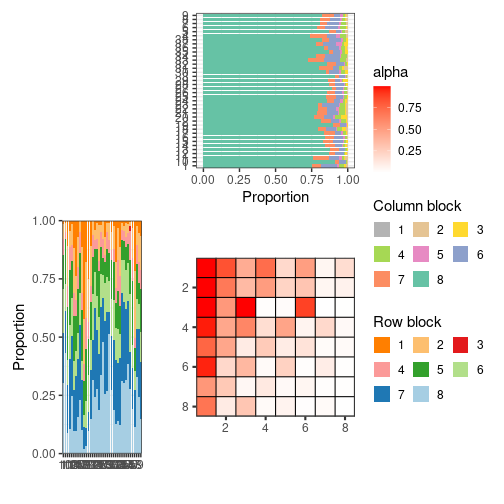
\includegraphics{figure/iid_meso_plot-1.png}
\caption{Collection 1 - iid}
\end{figure}

\begin{longtable}[]{@{}l@{}}
\toprule
Networks\tabularnewline
\midrule
\endhead
arroyo1982\_1+arroyo1982\_2+arroyo3\tabularnewline
eberling1999\tabularnewline
kato1990\tabularnewline
petanidou1991\tabularnewline
Junker2013\tabularnewline
bartomeus2008\tabularnewline
Benadi2013\_1(950m)+Benadi2013\_2(1170m)+Benadi2013\_6(2020m)\tabularnewline
Benadi2013\_4(1700m)+Benadi2013\_5(1800m)\tabularnewline
Struck1994\tabularnewline
Kato2000\tabularnewline
Albrecht2010\_49yr+Albrecht2010\_63yr+Albrecht2010\_84yr+Albrecht2010\_109yr+Albrecht2010\_130yr\tabularnewline
Baldock2011\_TB+Baldock2011\_JN\tabularnewline
Dattilo2016\tabularnewline
Devoto2005\_PP+Devoto2005\_AP\tabularnewline
Devoto2005\_VT\tabularnewline
Devoto2005\_LL+Devoto2005\_CT\tabularnewline
Freitas2006\tabularnewline
Gibson2006\_TA2\tabularnewline
Jedrzejewska2013\_Ochata+Jedrzejewska2013\_Kabaty\tabularnewline
MonteroCastano2017\_Albufera+MonteroCastano2017\_Llimpa+MonteroCastano2017\_Tirant\tabularnewline
Kehinde2014\_Joostenberg\_Conv+Kehinde2014\_Joostenberg\_Org+Kehinde2014\_Joostenberg\_Nat+Kehinde2014\_Laibach\_Conv+Kehinde2014\_Laibach\_Org+Kehinde2014\_Laibach\_Nat+Kehinde2014\_Spier\_Conv+Kehinde2014\_Spier\_Nat\tabularnewline
Pinheiro2008\tabularnewline
Watts2016\_Chicon+Watts2016\_Mantanay+Watts2016\_Choquebamba+Watts2016\_Huaran+Watts2016\_Piscacucho+Watts2016\_Poques+Watts2016\_Pumamarca+Watts2016\_Tiaparo+Watts2016\_Yanacocha\tabularnewline
Kato1993\tabularnewline
KatoMiura1996\tabularnewline
Kakutani1990\tabularnewline
Inoue1990\tabularnewline
Fragoso\_RA2+Fragoso\_RA3+Fragoso\_RD1+Fragoso\_RD3\tabularnewline
Souza\_cerrado\tabularnewline
Souza\_chaco\tabularnewline
Souza\_pantanal\tabularnewline
Souza\_vereda\tabularnewline
Adedoja2019\tabularnewline
Oleques2019\tabularnewline
Baldock2019\_Bristol\tabularnewline
Baldock2019\_Edinburgh\tabularnewline
Baldock2019\_Leeds\tabularnewline
Baldock2019\_Reading\tabularnewline
\bottomrule
\end{longtable}

Pour la collection 2

\begin{figure}
\centering
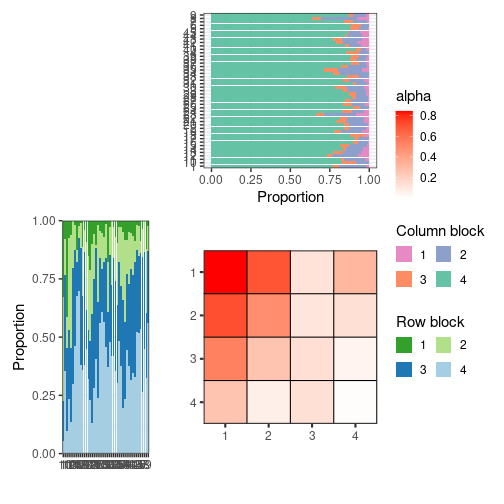
\includegraphics{figure/iid_meso_plot-2.png}
\caption{Collection 2 - iid}
\end{figure}

\begin{longtable}[]{@{}l@{}}
\toprule
Networks\tabularnewline
\midrule
\endhead
dupont2003\tabularnewline
herrera1988\tabularnewline
inouye1988\tabularnewline
medan2002ld\tabularnewline
medan2002rb\tabularnewline
ramirez1992\tabularnewline
ramirez1989\tabularnewline
Burkle2013\tabularnewline
Olito-Fox2014\tabularnewline
Benadi2013\_3(1340m)\tabularnewline
Aizen2008\_Challhuaco\_U+Aizen2008\_Challhuaco\_D\tabularnewline
Aizen2008\_Cerro Otto\_U+Aizen2008\_Cerro Otto\_D\tabularnewline
Aizen2008\_Llao-llao\_U+Aizen2008\_Llao-llao\_D\tabularnewline
Chamberlain\_cr1+Chamberlain\_cr2+Chamberlain\_fs1+Chamberlain\_fs2+Chamberlain\_go1+Chamberlain\_go2+Chamberlain\_mm1+Chamberlain\_mm2+Chamberlain\_mz1+Chamberlain\_mz2+Chamberlain\_sm1+Chamberlain\_sm2\tabularnewline
Chamberlain\_HLU+Chamberlain\_HLG+Chamberlain\_OKU+Chamberlain\_OKG+Chamberlain\_WLU+Chamberlain\_WLG+Chamberlain\_SOU+Chamberlain\_SOG\tabularnewline
Devoto2005\_LQ\tabularnewline
Devoto2005\_LT+Devoto2005\_LH\tabularnewline
LemusJimenez2003\tabularnewline
Lundgren2005\tabularnewline
Marrero2013\tabularnewline
Trojelsgaard2015\_La Gomera\tabularnewline
Trojelsgaard2015\_Gran Canaria\tabularnewline
Zackenberg\tabularnewline
Yoshihara2008\tabularnewline
Fragoso\_RA1+Fragoso\_RD2\tabularnewline
PopicThesis\tabularnewline
Pornon2017\tabularnewline
Orford\_B1+Orford\_B2+Orford\_B3+Orford\_B4+Orford\_B5+Orford\_B10\tabularnewline
Orford\_B6+Orford\_B7+Orford\_B8+Orford\_B9\tabularnewline
Blumel2016\tabularnewline
Kantsa2018\tabularnewline
Bennett2018\tabularnewline
Adedoja2018b\_baseZone+Adedoja2018b\_MidZone+Adedoja2018b\_HighZone+Adedoja2018b\_PeakZone\tabularnewline
CordenizPicanco2018\_NatVeg\tabularnewline
CordenizPicanco2018\_ExoFor\tabularnewline
Benadi2018\tabularnewline
Hackett2019\_NZ\_salt\_marsh+Hackett2019\_NZ\_sand\_dune+Hackett2019\_NZ\_scrub\_coprosma\tabularnewline
Jolls2019\tabularnewline
Traveset2013\_Fernandina\tabularnewline
Traveset2013\_Pinta\tabularnewline
Traveset2013\_Santiago\tabularnewline
Traveset2013\_SantaCruz\tabularnewline
Traveset2013\_SanCristobal\tabularnewline
Simanonok2014\tabularnewline
Son2019\_a1+Son2019\_a2+Son2019\_a3+Son2019\_a4+Son2019\_a5+Son2019\_a6+Son2019\_a7+Son2019\_a8+Son2019\_F1+Son2019\_F2+Son2019\_F3+Son2019\_F4+Son2019\_F5+Son2019\_F6+Son2019\_F7+Son2019\_F8\tabularnewline
\bottomrule
\end{longtable}

Pour la collection 3

\begin{figure}
\centering
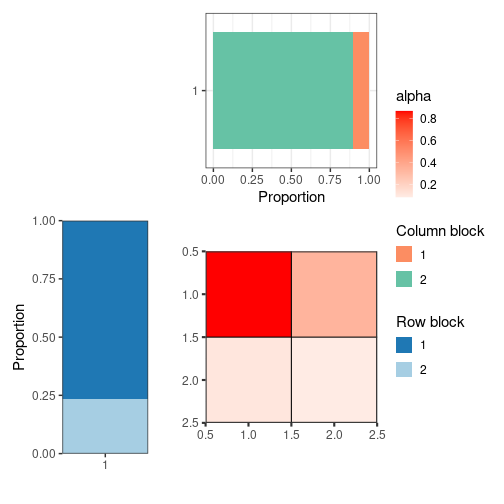
\includegraphics{figure/iid_meso_plot-3.png}
\caption{Collection 3 - iid}
\end{figure}

\begin{longtable}[]{@{}l@{}}
\toprule
Networks\tabularnewline
\midrule
\endhead
small1976\tabularnewline
\bottomrule
\end{longtable}

Pour la collection 4

\begin{figure}
\centering
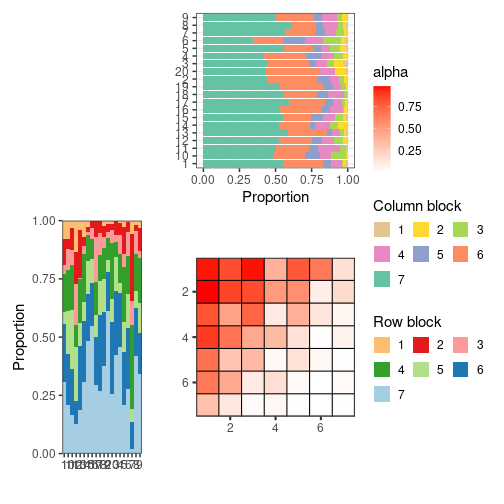
\includegraphics{figure/iid_meso_plot-4.png}
\caption{Collection 4 - iid}
\end{figure}

\begin{longtable}[]{@{}l@{}}
\toprule
Networks\tabularnewline
\midrule
\endhead
smith-ramirez2005\tabularnewline
Weiner2011\tabularnewline
Kaiser\_control+Kaiser\_restored\tabularnewline
Gilarranz2014\_amarante+Gilarranz2014\_barrosa+Gilarranz2014\_cincocerros+Gilarranz2014\_difuntito+Gilarranz2014\_difuntos+Gilarranz2014\_elmorro+Gilarranz2014\_labrava+Gilarranz2014\_lachata+Gilarranz2014\_lapaja+Gilarranz2014\_piedraalta+Gilarranz2014\_vigilancia+Gilarranz2014\_volcan\tabularnewline
Kaiser-Bunbury2017\_Bernica+Kaiser-Bunbury2017\_Casse-dent+Kaiser-Bunbury2017\_Copolia+Kaiser-Bunbury2017\_La-Reserve+Kaiser-Bunbury2017\_Rosebelle+Kaiser-Bunbury2017\_Salazie+Kaiser-Bunbury2017\_Tea-Plantation+Kaiser-Bunbury2017\_Trois-Freres\tabularnewline
Fang2012\tabularnewline
Aizen2008\_Puerto Blest\_U+Aizen2008\_Puerto Blest\_D\tabularnewline
Chamberlain\_Site1+Chamberlain\_Site2+Chamberlain\_Site3+Chamberlain\_Site4+Chamberlain\_Site5+Chamberlain\_Site6\tabularnewline
Dupont2009\_IsenBjerg+Dupont2009\_Other\tabularnewline
Gibson2006\_GA1\tabularnewline
Gibson2006\_TA1\tabularnewline
LaraRomero2016\_pe?alara\_EP+LaraRomero2016\_pe?alara\_PA+LaraRomero2016\_nevero\_EP+LaraRomero2016\_nevero\_PA\tabularnewline
Trojelsgaard2015\_Tenerife Teno Bajo+Trojelsgaard2015\_Tenerife
Fasnia\tabularnewline
Vanbergen2013\_balfarm+Vanbergen2013\_bridgend+Vanbergen2013\_dalhaikie+Vanbergen2013\_netherton+Vanbergen2013\_backhill+Vanbergen2013\_corntulloch+Vanbergen2013\_allancreich\tabularnewline
Pfeiffer\_CNE+Pfeiffer\_CNM+Pfeiffer\_CNT+Pfeiffer\_CPB+Pfeiffer\_CPM+Pfeiffer\_CPR+Pfeiffer\_CPS+Pfeiffer\_M2+Pfeiffer\_RP1+Pfeiffer\_RP2+Pfeiffer\_LM+Pfeiffer\_LO+Pfeiffer\_BD+Pfeiffer\_BH+Pfeiffer\_BS\tabularnewline
Carstensen\_Gigante+Carstensen\_Paulino+Carstensen\_Tinkerbell+Carstensen\_Midway+Carstensen\_Cedro+Carstensen\_Elefante+Carstensen\_Soizig\tabularnewline
Welti\_ID+Welti\_K1B+Welti\_K4A+Welti\_4B+Welti\_20B+Welti\_20C+Welti\_N1A+Welti\_N1B+Welti\_N4A+Welti\_N4B+Welti\_N20A+Welti\_N20B\tabularnewline
Grass2013\_1+Grass2013\_2+Grass2013\_3+Grass2013\_4+Grass2013\_5+Grass2013\_6+Grass2013\_7+Grass2013\_8+Grass2013\_9+Grass2013\_10+Grass2013\_11+Grass2013\_12+Grass2013\_13+Grass2013\_14+Grass2013\_15+Grass2013\_16+Grass2013\_17\tabularnewline
Hackett2019\_UK\_sand\_dune+Hackett2019\_UK\_grassland+Hackett2019\_UK\_heathland+Hackett2019\_UK\_woodland+Hackett2019\_UK\_salt\_marsh+Hackett2019\_UK\_scrub\tabularnewline
Neli2014\tabularnewline
\bottomrule
\end{longtable}

Pour la collection 5

\begin{figure}
\centering
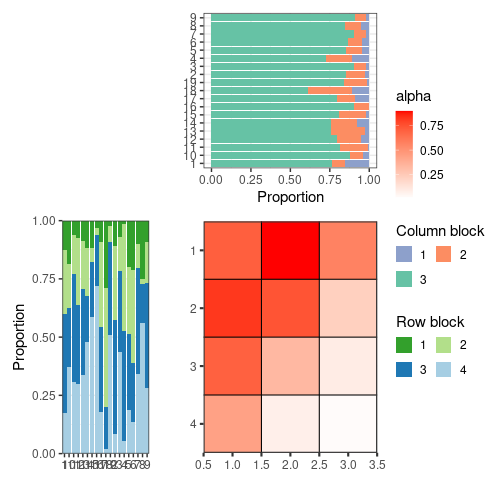
\includegraphics{figure/iid_meso_plot-5.png}
\caption{Collection 5 - iid}
\end{figure}

\begin{longtable}[]{@{}l@{}}
\toprule
Networks\tabularnewline
\midrule
\endhead
olensen2002aig\tabularnewline
olensen2002flo\tabularnewline
vazquez2002\tabularnewline
Shay2016\tabularnewline
Gibson2006\_GA2\tabularnewline
Gibson2006\_SG\tabularnewline
Trojelsgaard2015\_El Hierro\tabularnewline
Trojelsgaard2015\_Fuerteventura\tabularnewline
Trojelsgaard2015\_Western Sahara\tabularnewline
Robinson2018\tabularnewline
CordenizPicanco2018\_NatFor\tabularnewline
CordenizPicanco2018\_SemiPast\tabularnewline
CordenizPicanco2018\_IntPast\tabularnewline
Biella2019\tabularnewline
Nel2017\tabularnewline
Villalobos2019\tabularnewline
LaraRomero2019\_blanca+LaraRomero2019\_rajada+LaraRomero2019\_refugio+LaraRomero2019\_torre\tabularnewline
Ferrero2013\tabularnewline
Sritongchuay2019\_near+Sritongchuay2019\_far\tabularnewline
\bottomrule
\end{longtable}

Et voici donc les valeurs numériques pour les \(\alpha\) (paramètres de
connectivité).

Pour la collection 1 :
\[\begin{bmatrix} 1 &0.83 &0.43 &0.73 &0.2 &0.5 &0.05 &0.18 \\1 &0.67 &0.36 &0.51 &0.22 &0.3 &0.05 &0.07 \\1 &0.53 &1 &0.01 &0.02 &0.89 &0 &0 \\0.97 &0.45 &0.62 &0.18 &0.47 &0.06 &0.2 &0.03 \\0.76 &0.46 &0.1 &0.27 &0.1 &0.14 &0.02 &0.03 \\0.96 &0.2 &0.37 &0.03 &0.24 &0.01 &0.09 &0.01 \\0.54 &0.28 &0.04 &0.12 &0.03 &0.05 &0.01 &0.01 \\0.69 &0.1 &0.3 &0.02 &0.06 &0.01 &0.03 &0 \\ \end{bmatrix}\]
Pour la collection 2 :
\[\begin{bmatrix} 0.84 &0.69 &0.13 &0.32 \\0.71 &0.49 &0.11 &0.14 \\0.54 &0.26 &0.14 &0.05 \\0.26 &0.07 &0.14 &0.01 \\ \end{bmatrix}\]
Pour la collection 3 :
\[\begin{bmatrix} 0.87 &0.33 \\0.11 &0.09 \\ \end{bmatrix}\] Pour la
collection 4 :
\[\begin{bmatrix} 0.96 &0.83 &0.96 &0.39 &0.8 &0.16 &0.66 \\0.98 &0.86 &0.83 &0.51 &0.56 &0.19 &0.09 \\0.8 &0.46 &0.74 &0.12 &0.4 &0.05 &0.13 \\0.89 &0.69 &0.44 &0.35 &0.15 &0.07 &0.01 \\0.7 &0.29 &0.35 &0.03 &0.15 &0.01 &0.03 \\0.66 &0.43 &0.1 &0.17 &0.03 &0.02 &0 \\0.32 &0.12 &0.02 &0.04 &0 &0 &0 \\ \end{bmatrix}\]
Pour la collection 5 :
\[\begin{bmatrix} 0.71 &0.9 &0.57 &0.83 \\0.74 &0.22 &0.7 &0.33 \\0.09 &0.44 &0.07 &0.02 \\ \end{bmatrix}\]
\#\#\# Comparaison avec des infos supplémentaires

\begin{figure}
\centering
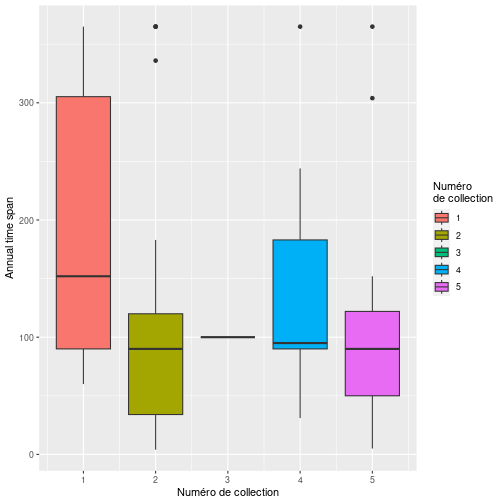
\includegraphics{figure/Annual_timespan_plot-1.png}
\caption{plot of chunk Annual\_timespan\_plot}
\end{figure}

\hypertarget{ruxe9partition-dans-les-clusters-selon-la-taxonomie}{%
\subsubsection{Répartition dans les clusters selon la
taxonomie}\label{ruxe9partition-dans-les-clusters-selon-la-taxonomie}}

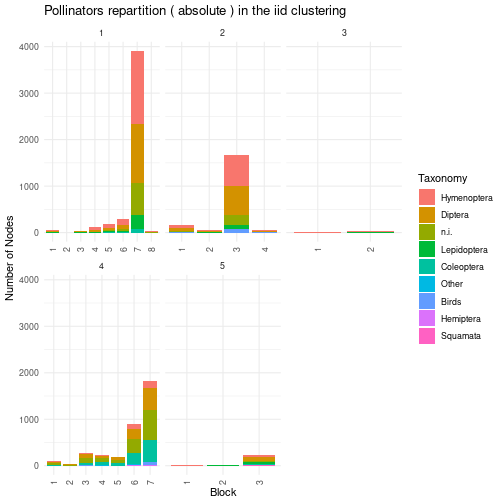
\includegraphics{figure/iid_plot_taxonomy_pollinators-1.png}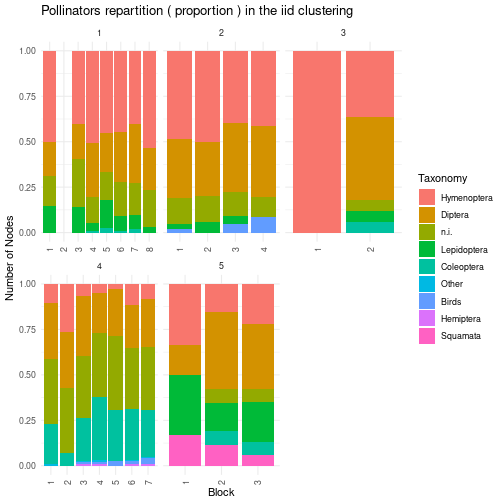
\includegraphics{figure/iid_plot_taxonomy_pollinators-2.png}

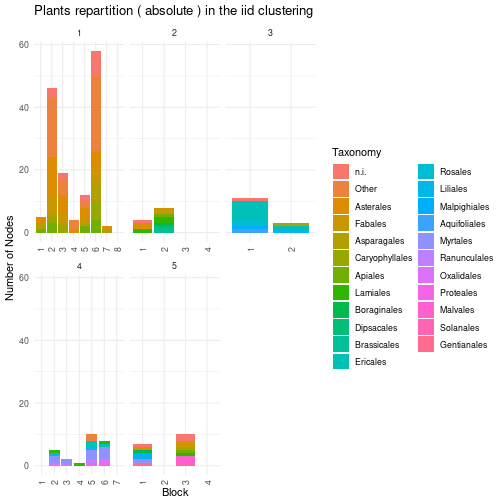
\includegraphics{figure/iid_plot_taxonomy_plants-1.png}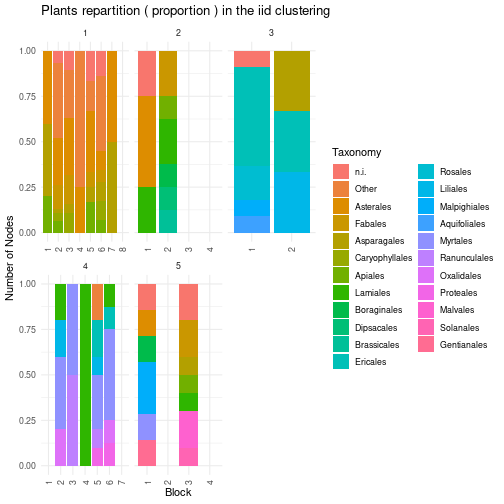
\includegraphics{figure/iid_plot_taxonomy_plants-2.png}

\hypertarget{tables}{%
\paragraph{Tables}\label{tables}}

\begin{verbatim}
## # A tibble: 9 × 25
##   Taxon       Collection_1_Bloc_1 Collection_1_Bloc_2 Collection_1_Bloc_3
##   <fct>                     <dbl>               <dbl>               <dbl>
## 1 Hymenoptera                  24                   0                  17
## 2 Diptera                       9                   0                   8
## 3 n.i.                          8                   0                  11
## 4 Lepidoptera                   7                   0                   6
## 5 Coleoptera                    0                   0                   0
## 6 Other                         0                   0                   0
## 7 Birds                        NA                  NA                  NA
## 8 Hemiptera                    NA                  NA                  NA
## 9 Squamata                     NA                  NA                  NA
## # ℹ 21 more variables: Collection_1_Bloc_4 <dbl>, Collection_1_Bloc_5 <dbl>,
## #   Collection_1_Bloc_6 <dbl>, Collection_1_Bloc_7 <dbl>,
## #   Collection_1_Bloc_8 <dbl>, Collection_2_Bloc_1 <dbl>,
## #   Collection_2_Bloc_2 <dbl>, Collection_2_Bloc_3 <dbl>,
## #   Collection_2_Bloc_4 <dbl>, Collection_3_Bloc_1 <dbl>,
## #   Collection_3_Bloc_2 <dbl>, Collection_4_Bloc_1 <dbl>,
## #   Collection_4_Bloc_2 <dbl>, Collection_4_Bloc_3 <dbl>, …
\end{verbatim}

\hypertarget{clustering-avec-le-moduxe8le-pi}{%
\subsection{Clustering avec le modèle
pi}\label{clustering-avec-le-moduxe8le-pi}}

Avec le modèle \emph{pi} nous obtenons les 2 collections et les
structures suivantes:

Pour la collection 1

\begin{figure}
\centering
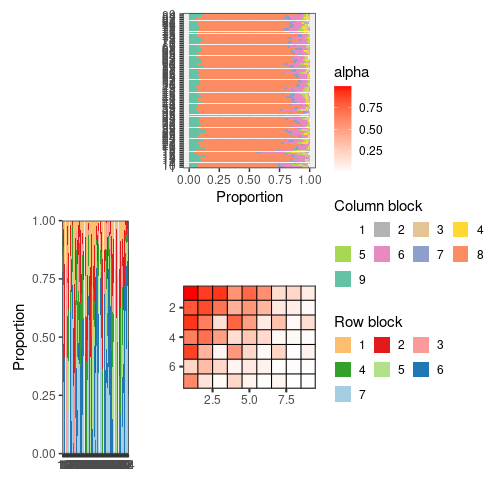
\includegraphics{figure/pi_meso_plot-1.png}
\caption{Collection 1 - pi}
\end{figure}

\begin{longtable}[]{@{}l@{}}
\toprule
Networks\tabularnewline
\midrule
\endhead
arroyo1982\_1+arroyo1982\_2+arroyo3\tabularnewline
eberling1999\tabularnewline
inouye1988\tabularnewline
kato1990\tabularnewline
ramirez1992\tabularnewline
petanidou1991\tabularnewline
ramirez1989\tabularnewline
smith-ramirez2005\tabularnewline
Junker2013\tabularnewline
Kaiser\_control+Kaiser\_restored\tabularnewline
bartomeus2008\tabularnewline
Olito-Fox2014\tabularnewline
Benadi2013\_1(950m)+Benadi2013\_2(1170m)+Benadi2013\_6(2020m)\tabularnewline
Benadi2013\_3(1340m)\tabularnewline
Benadi2013\_4(1700m)+Benadi2013\_5(1800m)\tabularnewline
Kaiser-Bunbury2017\_Bernica+Kaiser-Bunbury2017\_Casse-dent+Kaiser-Bunbury2017\_Copolia+Kaiser-Bunbury2017\_La-Reserve+Kaiser-Bunbury2017\_Rosebelle+Kaiser-Bunbury2017\_Salazie+Kaiser-Bunbury2017\_Tea-Plantation+Kaiser-Bunbury2017\_Trois-Freres\tabularnewline
Fang2012\tabularnewline
Shay2016\tabularnewline
Struck1994\tabularnewline
Kato2000\tabularnewline
Aizen2008\_Cerro Otto\_U+Aizen2008\_Cerro Otto\_D\tabularnewline
Aizen2008\_Llao-llao\_U+Aizen2008\_Llao-llao\_D\tabularnewline
Aizen2008\_Puerto Blest\_U+Aizen2008\_Puerto Blest\_D\tabularnewline
Albrecht2010\_49yr+Albrecht2010\_63yr+Albrecht2010\_84yr+Albrecht2010\_109yr+Albrecht2010\_130yr\tabularnewline
Baldock2011\_TB+Baldock2011\_JN\tabularnewline
Chamberlain\_cr1+Chamberlain\_cr2+Chamberlain\_fs1+Chamberlain\_fs2+Chamberlain\_go1+Chamberlain\_go2+Chamberlain\_mm1+Chamberlain\_mm2+Chamberlain\_mz1+Chamberlain\_mz2+Chamberlain\_sm1+Chamberlain\_sm2\tabularnewline
Chamberlain\_HLU+Chamberlain\_HLG+Chamberlain\_OKU+Chamberlain\_OKG+Chamberlain\_WLU+Chamberlain\_WLG+Chamberlain\_SOU+Chamberlain\_SOG\tabularnewline
Chamberlain\_Site1+Chamberlain\_Site2+Chamberlain\_Site3+Chamberlain\_Site4+Chamberlain\_Site5+Chamberlain\_Site6\tabularnewline
Dattilo2016\tabularnewline
Devoto2005\_PP+Devoto2005\_AP\tabularnewline
Devoto2005\_VT\tabularnewline
Devoto2005\_LL+Devoto2005\_CT\tabularnewline
Dupont2009\_IsenBjerg+Dupont2009\_Other\tabularnewline
Freitas2006\tabularnewline
Gibson2006\_TA1\tabularnewline
Gibson2006\_TA2\tabularnewline
Jedrzejewska2013\_Ochata+Jedrzejewska2013\_Kabaty\tabularnewline
LaraRomero2016\_pe?alara\_EP+LaraRomero2016\_pe?alara\_PA+LaraRomero2016\_nevero\_EP+LaraRomero2016\_nevero\_PA\tabularnewline
LemusJimenez2003\tabularnewline
Marrero2013\tabularnewline
MonteroCastano2017\_Albufera+MonteroCastano2017\_Llimpa+MonteroCastano2017\_Tirant\tabularnewline
Kehinde2014\_Joostenberg\_Conv+Kehinde2014\_Joostenberg\_Org+Kehinde2014\_Joostenberg\_Nat+Kehinde2014\_Laibach\_Conv+Kehinde2014\_Laibach\_Org+Kehinde2014\_Laibach\_Nat+Kehinde2014\_Spier\_Conv+Kehinde2014\_Spier\_Nat\tabularnewline
Pinheiro2008\tabularnewline
Trojelsgaard2015\_La Gomera\tabularnewline
Trojelsgaard2015\_Tenerife Teno Bajo+Trojelsgaard2015\_Tenerife
Fasnia\tabularnewline
Vanbergen2013\_balfarm+Vanbergen2013\_bridgend+Vanbergen2013\_dalhaikie+Vanbergen2013\_netherton+Vanbergen2013\_backhill+Vanbergen2013\_corntulloch+Vanbergen2013\_allancreich\tabularnewline
Zackenberg\tabularnewline
Yoshihara2008\tabularnewline
Watts2016\_Chicon+Watts2016\_Mantanay+Watts2016\_Choquebamba+Watts2016\_Huaran+Watts2016\_Piscacucho+Watts2016\_Poques+Watts2016\_Pumamarca+Watts2016\_Tiaparo+Watts2016\_Yanacocha\tabularnewline
Kato1993\tabularnewline
KatoMiura1996\tabularnewline
Kakutani1990\tabularnewline
Inoue1990\tabularnewline
Fragoso\_RA2+Fragoso\_RA3+Fragoso\_RD1+Fragoso\_RD3\tabularnewline
PopicThesis\tabularnewline
Pfeiffer\_CNE+Pfeiffer\_CNM+Pfeiffer\_CNT+Pfeiffer\_CPB+Pfeiffer\_CPM+Pfeiffer\_CPR+Pfeiffer\_CPS+Pfeiffer\_M2+Pfeiffer\_RP1+Pfeiffer\_RP2+Pfeiffer\_LM+Pfeiffer\_LO+Pfeiffer\_BD+Pfeiffer\_BH+Pfeiffer\_BS\tabularnewline
Carstensen\_Gigante+Carstensen\_Paulino+Carstensen\_Tinkerbell+Carstensen\_Midway+Carstensen\_Cedro+Carstensen\_Elefante+Carstensen\_Soizig\tabularnewline
Orford\_B1+Orford\_B2+Orford\_B3+Orford\_B4+Orford\_B5+Orford\_B10\tabularnewline
Orford\_B6+Orford\_B7+Orford\_B8+Orford\_B9\tabularnewline
Blumel2016\tabularnewline
Welti\_ID+Welti\_K1B+Welti\_K4A+Welti\_4B+Welti\_20B+Welti\_20C+Welti\_N1A+Welti\_N1B+Welti\_N4A+Welti\_N4B+Welti\_N20A+Welti\_N20B\tabularnewline
Souza\_cerrado\tabularnewline
Souza\_chaco\tabularnewline
Souza\_pantanal\tabularnewline
Souza\_vereda\tabularnewline
Grass2013\_1+Grass2013\_2+Grass2013\_3+Grass2013\_4+Grass2013\_5+Grass2013\_6+Grass2013\_7+Grass2013\_8+Grass2013\_9+Grass2013\_10+Grass2013\_11+Grass2013\_12+Grass2013\_13+Grass2013\_14+Grass2013\_15+Grass2013\_16+Grass2013\_17\tabularnewline
Bennett2018\tabularnewline
Adedoja2018b\_baseZone+Adedoja2018b\_MidZone+Adedoja2018b\_HighZone+Adedoja2018b\_PeakZone\tabularnewline
Adedoja2019\tabularnewline
CordenizPicanco2018\_NatVeg\tabularnewline
Benadi2018\tabularnewline
Hackett2019\_NZ\_salt\_marsh+Hackett2019\_NZ\_sand\_dune+Hackett2019\_NZ\_scrub\_coprosma\tabularnewline
Oleques2019\tabularnewline
Jolls2019\tabularnewline
Traveset2013\_Fernandina\tabularnewline
Traveset2013\_Santiago\tabularnewline
Traveset2013\_SantaCruz\tabularnewline
Traveset2013\_SanCristobal\tabularnewline
Simanonok2014\tabularnewline
Son2019\_a1+Son2019\_a2+Son2019\_a3+Son2019\_a4+Son2019\_a5+Son2019\_a6+Son2019\_a7+Son2019\_a8+Son2019\_F1+Son2019\_F2+Son2019\_F3+Son2019\_F4+Son2019\_F5+Son2019\_F6+Son2019\_F7+Son2019\_F8\tabularnewline
Baldock2019\_Bristol\tabularnewline
Baldock2019\_Edinburgh\tabularnewline
Baldock2019\_Leeds\tabularnewline
Baldock2019\_Reading\tabularnewline
\bottomrule
\end{longtable}

Pour la collection 2

\begin{figure}
\centering
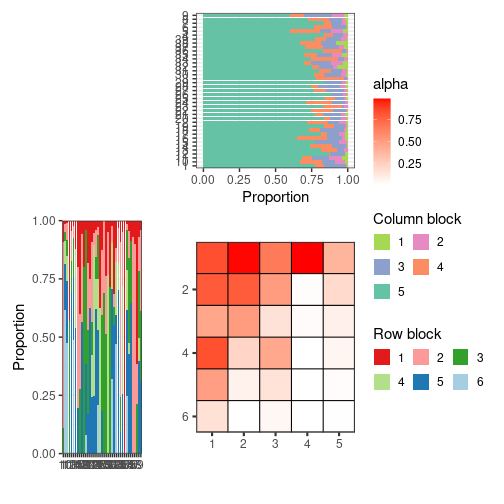
\includegraphics{figure/pi_meso_plot-2.png}
\caption{Collection 2 - pi}
\end{figure}

\begin{longtable}[]{@{}l@{}}
\toprule
Networks\tabularnewline
\midrule
\endhead
dupont2003\tabularnewline
herrera1988\tabularnewline
medan2002ld\tabularnewline
medan2002rb\tabularnewline
olensen2002aig\tabularnewline
olensen2002flo\tabularnewline
small1976\tabularnewline
vazquez2002\tabularnewline
Burkle2013\tabularnewline
Weiner2011\tabularnewline
Gilarranz2014\_amarante+Gilarranz2014\_barrosa+Gilarranz2014\_cincocerros+Gilarranz2014\_difuntito+Gilarranz2014\_difuntos+Gilarranz2014\_elmorro+Gilarranz2014\_labrava+Gilarranz2014\_lachata+Gilarranz2014\_lapaja+Gilarranz2014\_piedraalta+Gilarranz2014\_vigilancia+Gilarranz2014\_volcan\tabularnewline
Aizen2008\_Challhuaco\_U+Aizen2008\_Challhuaco\_D\tabularnewline
Devoto2005\_LQ\tabularnewline
Devoto2005\_LT+Devoto2005\_LH\tabularnewline
Gibson2006\_GA1\tabularnewline
Gibson2006\_GA2\tabularnewline
Gibson2006\_SG\tabularnewline
Lundgren2005\tabularnewline
Trojelsgaard2015\_El Hierro\tabularnewline
Trojelsgaard2015\_Gran Canaria\tabularnewline
Trojelsgaard2015\_Fuerteventura\tabularnewline
Trojelsgaard2015\_Western Sahara\tabularnewline
Fragoso\_RA1+Fragoso\_RD2\tabularnewline
Pornon2017\tabularnewline
Kantsa2018\tabularnewline
Robinson2018\tabularnewline
CordenizPicanco2018\_NatFor\tabularnewline
CordenizPicanco2018\_ExoFor\tabularnewline
CordenizPicanco2018\_SemiPast\tabularnewline
CordenizPicanco2018\_IntPast\tabularnewline
Hackett2019\_UK\_sand\_dune+Hackett2019\_UK\_grassland+Hackett2019\_UK\_heathland+Hackett2019\_UK\_woodland+Hackett2019\_UK\_salt\_marsh+Hackett2019\_UK\_scrub\tabularnewline
Biella2019\tabularnewline
Nel2017\tabularnewline
Villalobos2019\tabularnewline
LaraRomero2019\_blanca+LaraRomero2019\_rajada+LaraRomero2019\_refugio+LaraRomero2019\_torre\tabularnewline
Traveset2013\_Pinta\tabularnewline
Ferrero2013\tabularnewline
Neli2014\tabularnewline
Sritongchuay2019\_near+Sritongchuay2019\_far\tabularnewline
\bottomrule
\end{longtable}

Et voici donc les valeurs numériques pour les \(\alpha\) (paramètres de
connectivité).

Pour la collection 1 :
\[\begin{bmatrix} 1 &0.9 &0.92 &0.55 &0.75 &0.57 &0.17 \\0.1 &0.21 &0.81 &0.86 &0.7 &0.4 &0.54 \\0.38 &0.12 &0.03 &0.09 &0.92 &0.65 &0.17 \\0.76 &0.5 &0.1 &0.33 &0.17 &0.04 &0.65 \\0.71 &0.5 &0.18 &0.28 &0.19 &0.04 &0.01 \\0.03 &0.89 &0.4 &0.05 &0.53 &0.2 &0.03 \\0.22 &0.07 &0.01 &0.22 &0.35 &0.21 &0.06 \\0.11 &0.07 &0.01 &0.01 &0.01 &0.6 &0.15 \\0.02 &0.21 &0.06 &0.01 &0.06 &0.01 &0 \\ \end{bmatrix}\]
Pour la collection 2 :
\[\begin{bmatrix} 0.84 &0.99 &0.66 &0.99 &0.38 &0.79 \\0.79 &0.5 &0.01 &0.19 &0.46 &0.51 \\0.15 &0.02 &0.08 &0.83 &0.22 &0.44 \\0 &0.05 &0.49 &0.07 &0.15 &0 \\0.01 &0.16 &0 &0.04 &0 &0 \\ \end{bmatrix}\]

\hypertarget{ruxe9partition-dans-les-clusters-selon-la-taxonomie-1}{%
\subsubsection{Répartition dans les clusters selon la
taxonomie}\label{ruxe9partition-dans-les-clusters-selon-la-taxonomie-1}}

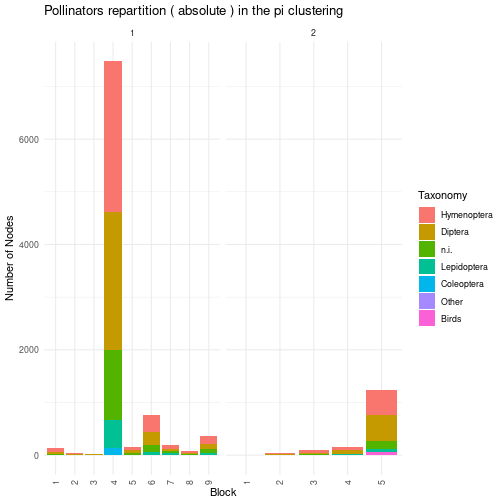
\includegraphics{figure/pi_plot_taxonomy_pollinators-1.png}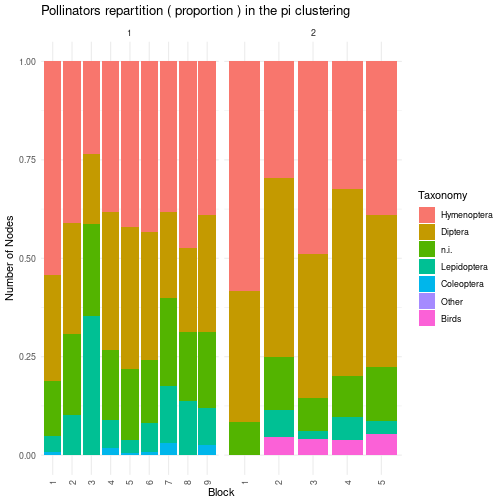
\includegraphics{figure/pi_plot_taxonomy_pollinators-2.png}

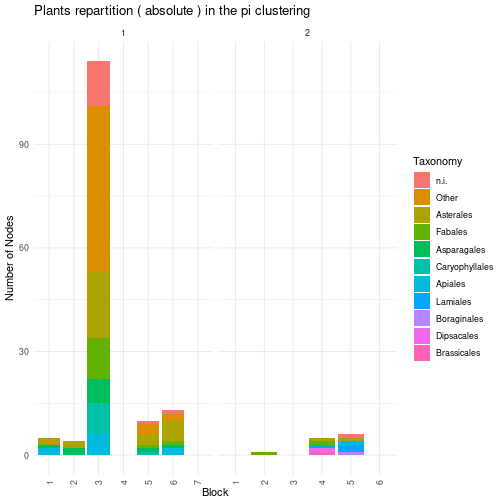
\includegraphics{figure/pi_plot_taxonomy_plants-1.png}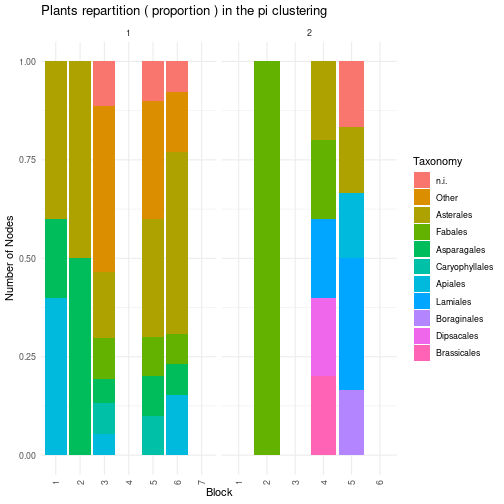
\includegraphics{figure/pi_plot_taxonomy_plants-2.png}

\hypertarget{clustering-avec-le-moduxe8le-rho}{%
\subsection{Clustering avec le modèle
rho}\label{clustering-avec-le-moduxe8le-rho}}

Avec le modèle \emph{rho} nous obtenons les 1 collections et les
structures suivantes:

Pour la collection 1

\begin{figure}
\centering
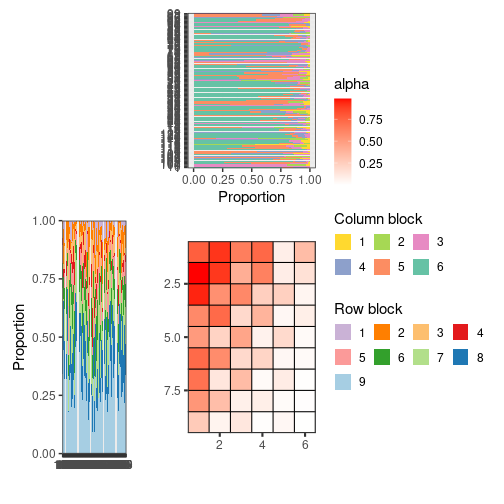
\includegraphics{figure/rho_meso_plot-1.png}
\caption{Collection 1 - rho}
\end{figure}

\begin{longtable}[]{@{}l@{}}
\toprule
Networks\tabularnewline
\midrule
\endhead
arroyo1982\_1+arroyo1982\_2+arroyo3\tabularnewline
dupont2003\tabularnewline
eberling1999\tabularnewline
herrera1988\tabularnewline
inouye1988\tabularnewline
kato1990\tabularnewline
medan2002ld\tabularnewline
medan2002rb\tabularnewline
olensen2002aig\tabularnewline
olensen2002flo\tabularnewline
ramirez1992\tabularnewline
small1976\tabularnewline
vazquez2002\tabularnewline
petanidou1991\tabularnewline
ramirez1989\tabularnewline
smith-ramirez2005\tabularnewline
Burkle2013\tabularnewline
Junker2013\tabularnewline
Weiner2011\tabularnewline
Kaiser\_control+Kaiser\_restored\tabularnewline
bartomeus2008\tabularnewline
Olito-Fox2014\tabularnewline
Gilarranz2014\_amarante+Gilarranz2014\_barrosa+Gilarranz2014\_cincocerros+Gilarranz2014\_difuntito+Gilarranz2014\_difuntos+Gilarranz2014\_elmorro+Gilarranz2014\_labrava+Gilarranz2014\_lachata+Gilarranz2014\_lapaja+Gilarranz2014\_piedraalta+Gilarranz2014\_vigilancia+Gilarranz2014\_volcan\tabularnewline
Benadi2013\_1(950m)+Benadi2013\_2(1170m)+Benadi2013\_6(2020m)\tabularnewline
Benadi2013\_3(1340m)\tabularnewline
Benadi2013\_4(1700m)+Benadi2013\_5(1800m)\tabularnewline
Kaiser-Bunbury2017\_Bernica+Kaiser-Bunbury2017\_Casse-dent+Kaiser-Bunbury2017\_Copolia+Kaiser-Bunbury2017\_La-Reserve+Kaiser-Bunbury2017\_Rosebelle+Kaiser-Bunbury2017\_Salazie+Kaiser-Bunbury2017\_Tea-Plantation+Kaiser-Bunbury2017\_Trois-Freres\tabularnewline
Fang2012\tabularnewline
Shay2016\tabularnewline
Struck1994\tabularnewline
Kato2000\tabularnewline
Aizen2008\_Challhuaco\_U+Aizen2008\_Challhuaco\_D\tabularnewline
Aizen2008\_Cerro Otto\_U+Aizen2008\_Cerro Otto\_D\tabularnewline
Aizen2008\_Llao-llao\_U+Aizen2008\_Llao-llao\_D\tabularnewline
Aizen2008\_Puerto Blest\_U+Aizen2008\_Puerto Blest\_D\tabularnewline
Albrecht2010\_49yr+Albrecht2010\_63yr+Albrecht2010\_84yr+Albrecht2010\_109yr+Albrecht2010\_130yr\tabularnewline
Baldock2011\_TB+Baldock2011\_JN\tabularnewline
Chamberlain\_cr1+Chamberlain\_cr2+Chamberlain\_fs1+Chamberlain\_fs2+Chamberlain\_go1+Chamberlain\_go2+Chamberlain\_mm1+Chamberlain\_mm2+Chamberlain\_mz1+Chamberlain\_mz2+Chamberlain\_sm1+Chamberlain\_sm2\tabularnewline
Chamberlain\_HLU+Chamberlain\_HLG+Chamberlain\_OKU+Chamberlain\_OKG+Chamberlain\_WLU+Chamberlain\_WLG+Chamberlain\_SOU+Chamberlain\_SOG\tabularnewline
Chamberlain\_Site1+Chamberlain\_Site2+Chamberlain\_Site3+Chamberlain\_Site4+Chamberlain\_Site5+Chamberlain\_Site6\tabularnewline
Dattilo2016\tabularnewline
Devoto2005\_LQ\tabularnewline
Devoto2005\_PP+Devoto2005\_AP\tabularnewline
Devoto2005\_LT+Devoto2005\_LH\tabularnewline
Devoto2005\_VT\tabularnewline
Devoto2005\_LL+Devoto2005\_CT\tabularnewline
Dupont2009\_IsenBjerg+Dupont2009\_Other\tabularnewline
Freitas2006\tabularnewline
Gibson2006\_GA1\tabularnewline
Gibson2006\_GA2\tabularnewline
Gibson2006\_SG\tabularnewline
Gibson2006\_TA1\tabularnewline
Gibson2006\_TA2\tabularnewline
Jedrzejewska2013\_Ochata+Jedrzejewska2013\_Kabaty\tabularnewline
LaraRomero2016\_pe?alara\_EP+LaraRomero2016\_pe?alara\_PA+LaraRomero2016\_nevero\_EP+LaraRomero2016\_nevero\_PA\tabularnewline
LemusJimenez2003\tabularnewline
Lundgren2005\tabularnewline
Marrero2013\tabularnewline
MonteroCastano2017\_Albufera+MonteroCastano2017\_Llimpa+MonteroCastano2017\_Tirant\tabularnewline
Kehinde2014\_Joostenberg\_Conv+Kehinde2014\_Joostenberg\_Org+Kehinde2014\_Joostenberg\_Nat+Kehinde2014\_Laibach\_Conv+Kehinde2014\_Laibach\_Org+Kehinde2014\_Laibach\_Nat+Kehinde2014\_Spier\_Conv+Kehinde2014\_Spier\_Nat\tabularnewline
Pinheiro2008\tabularnewline
Trojelsgaard2015\_El Hierro\tabularnewline
Trojelsgaard2015\_La Gomera\tabularnewline
Trojelsgaard2015\_Gran Canaria\tabularnewline
Trojelsgaard2015\_Fuerteventura\tabularnewline
Trojelsgaard2015\_Tenerife Teno Bajo+Trojelsgaard2015\_Tenerife
Fasnia\tabularnewline
Trojelsgaard2015\_Western Sahara\tabularnewline
Vanbergen2013\_balfarm+Vanbergen2013\_bridgend+Vanbergen2013\_dalhaikie+Vanbergen2013\_netherton+Vanbergen2013\_backhill+Vanbergen2013\_corntulloch+Vanbergen2013\_allancreich\tabularnewline
Zackenberg\tabularnewline
Yoshihara2008\tabularnewline
Watts2016\_Chicon+Watts2016\_Mantanay+Watts2016\_Choquebamba+Watts2016\_Huaran+Watts2016\_Piscacucho+Watts2016\_Poques+Watts2016\_Pumamarca+Watts2016\_Tiaparo+Watts2016\_Yanacocha\tabularnewline
Kato1993\tabularnewline
KatoMiura1996\tabularnewline
Kakutani1990\tabularnewline
Inoue1990\tabularnewline
Fragoso\_RA1+Fragoso\_RD2\tabularnewline
Fragoso\_RA2+Fragoso\_RA3+Fragoso\_RD1+Fragoso\_RD3\tabularnewline
PopicThesis\tabularnewline
Pfeiffer\_CNE+Pfeiffer\_CNM+Pfeiffer\_CNT+Pfeiffer\_CPB+Pfeiffer\_CPM+Pfeiffer\_CPR+Pfeiffer\_CPS+Pfeiffer\_M2+Pfeiffer\_RP1+Pfeiffer\_RP2+Pfeiffer\_LM+Pfeiffer\_LO+Pfeiffer\_BD+Pfeiffer\_BH+Pfeiffer\_BS\tabularnewline
Carstensen\_Gigante+Carstensen\_Paulino+Carstensen\_Tinkerbell+Carstensen\_Midway+Carstensen\_Cedro+Carstensen\_Elefante+Carstensen\_Soizig\tabularnewline
Pornon2017\tabularnewline
Orford\_B1+Orford\_B2+Orford\_B3+Orford\_B4+Orford\_B5+Orford\_B10\tabularnewline
Orford\_B6+Orford\_B7+Orford\_B8+Orford\_B9\tabularnewline
Blumel2016\tabularnewline
Welti\_ID+Welti\_K1B+Welti\_K4A+Welti\_4B+Welti\_20B+Welti\_20C+Welti\_N1A+Welti\_N1B+Welti\_N4A+Welti\_N4B+Welti\_N20A+Welti\_N20B\tabularnewline
Kantsa2018\tabularnewline
Souza\_cerrado\tabularnewline
Souza\_chaco\tabularnewline
Souza\_pantanal\tabularnewline
Souza\_vereda\tabularnewline
Grass2013\_1+Grass2013\_2+Grass2013\_3+Grass2013\_4+Grass2013\_5+Grass2013\_6+Grass2013\_7+Grass2013\_8+Grass2013\_9+Grass2013\_10+Grass2013\_11+Grass2013\_12+Grass2013\_13+Grass2013\_14+Grass2013\_15+Grass2013\_16+Grass2013\_17\tabularnewline
Robinson2018\tabularnewline
Bennett2018\tabularnewline
Adedoja2018b\_baseZone+Adedoja2018b\_MidZone+Adedoja2018b\_HighZone+Adedoja2018b\_PeakZone\tabularnewline
Adedoja2019\tabularnewline
CordenizPicanco2018\_NatFor\tabularnewline
CordenizPicanco2018\_NatVeg\tabularnewline
CordenizPicanco2018\_ExoFor\tabularnewline
CordenizPicanco2018\_SemiPast\tabularnewline
CordenizPicanco2018\_IntPast\tabularnewline
Benadi2018\tabularnewline
Hackett2019\_NZ\_salt\_marsh+Hackett2019\_NZ\_sand\_dune+Hackett2019\_NZ\_scrub\_coprosma\tabularnewline
Hackett2019\_UK\_sand\_dune+Hackett2019\_UK\_grassland+Hackett2019\_UK\_heathland+Hackett2019\_UK\_woodland+Hackett2019\_UK\_salt\_marsh+Hackett2019\_UK\_scrub\tabularnewline
Oleques2019\tabularnewline
Biella2019\tabularnewline
Jolls2019\tabularnewline
Nel2017\tabularnewline
Villalobos2019\tabularnewline
LaraRomero2019\_blanca+LaraRomero2019\_rajada+LaraRomero2019\_refugio+LaraRomero2019\_torre\tabularnewline
Traveset2013\_Fernandina\tabularnewline
Traveset2013\_Pinta\tabularnewline
Traveset2013\_Santiago\tabularnewline
Traveset2013\_SantaCruz\tabularnewline
Traveset2013\_SanCristobal\tabularnewline
Ferrero2013\tabularnewline
Simanonok2014\tabularnewline
Son2019\_a1+Son2019\_a2+Son2019\_a3+Son2019\_a4+Son2019\_a5+Son2019\_a6+Son2019\_a7+Son2019\_a8+Son2019\_F1+Son2019\_F2+Son2019\_F3+Son2019\_F4+Son2019\_F5+Son2019\_F6+Son2019\_F7+Son2019\_F8\tabularnewline
Neli2014\tabularnewline
Sritongchuay2019\_near+Sritongchuay2019\_far\tabularnewline
Baldock2019\_Bristol\tabularnewline
Baldock2019\_Edinburgh\tabularnewline
Baldock2019\_Leeds\tabularnewline
Baldock2019\_Reading\tabularnewline
\bottomrule
\end{longtable}

Et voici donc les valeurs numériques pour les \(\alpha\) (paramètres de
connectivité).

Pour la collection 1 :
\[\begin{bmatrix} 0.77 &0.91 &0.64 &0.73 &0.09 &0.34 &0.98 &0.9 &0.41 \\0.63 &0.09 &0.15 &0.94 &0.56 &0.6 &0.25 &0.24 &0.05 \\0.59 &0.73 &0.19 &0.38 &0.04 &0.09 &0.51 &0.22 &0.46 \\0.07 &0.19 &0.02 &0.73 &0.58 &0.2 &0.22 &0.04 &0.03 \\0.69 &0.13 &0.34 &0.03 &0.1 &0.01 &0.53 &0.33 &0.08 \\0.09 &0.02 &0.01 &0.27 &0.06 &0.12 &0.01 &0.04 &0 \\ \end{bmatrix}\]

\hypertarget{ruxe9partition-dans-les-clusters-selon-la-taxonomie-2}{%
\subsubsection{Répartition dans les clusters selon la
taxonomie}\label{ruxe9partition-dans-les-clusters-selon-la-taxonomie-2}}

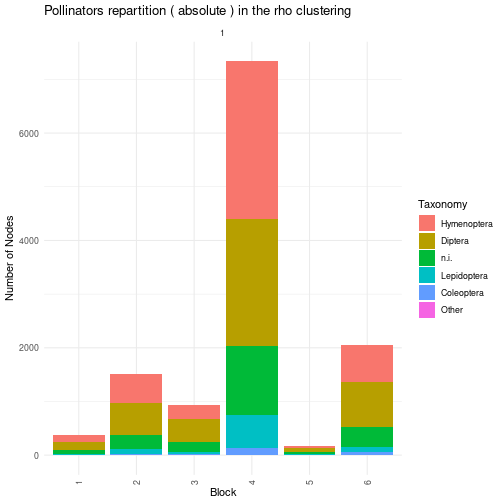
\includegraphics{figure/rho_plot_taxonomy_pollinators-1.png}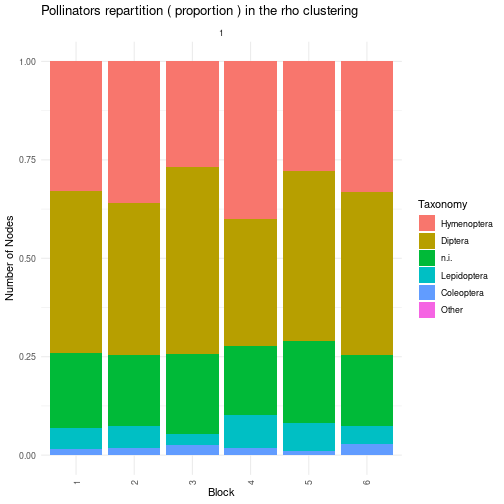
\includegraphics{figure/rho_plot_taxonomy_pollinators-2.png}

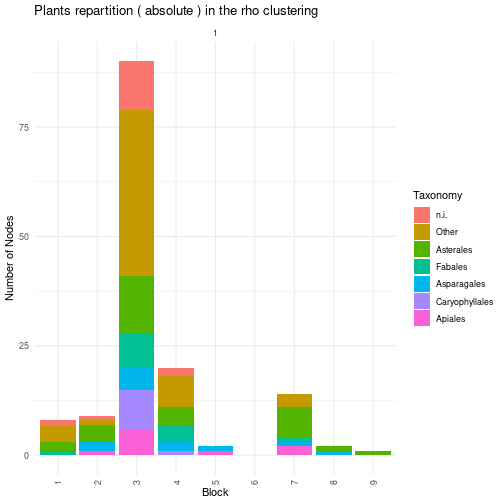
\includegraphics{figure/rho_plot_taxonomy_plants-1.png}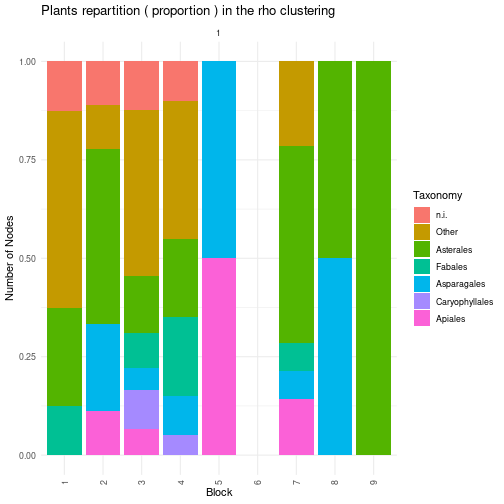
\includegraphics{figure/rho_plot_taxonomy_plants-2.png}

\hypertarget{clustering-avec-le-moduxe8le-pirho}{%
\subsection{Clustering avec le modèle
pirho}\label{clustering-avec-le-moduxe8le-pirho}}

Avec le modèle \emph{pirho} nous obtenons les 15 collections et les
structures suivantes:

Pour la collection 1

\begin{figure}
\centering
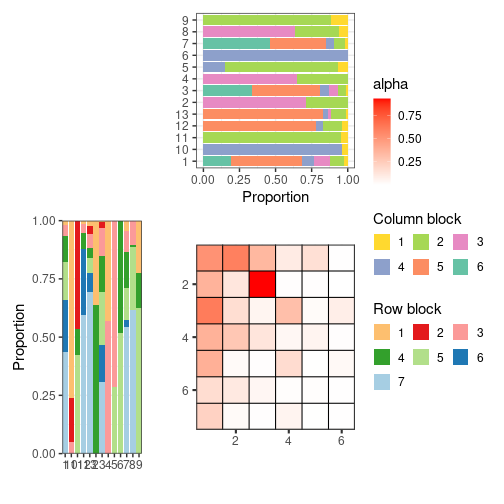
\includegraphics{figure/pirho_meso_plot-1.png}
\caption{Collection 1 - pirho}
\end{figure}

\begin{longtable}[]{@{}l@{}}
\toprule
Networks\tabularnewline
\midrule
\endhead
arroyo1982\_1+arroyo1982\_2+arroyo3\tabularnewline
dupont2003\tabularnewline
petanidou1991\tabularnewline
Aizen2008\_Challhuaco\_U+Aizen2008\_Challhuaco\_D\tabularnewline
Aizen2008\_Llao-llao\_U+Aizen2008\_Llao-llao\_D\tabularnewline
Jedrzejewska2013\_Ochata+Jedrzejewska2013\_Kabaty\tabularnewline
Pinheiro2008\tabularnewline
Souza\_pantanal\tabularnewline
Robinson2018\tabularnewline
Jolls2019\tabularnewline
Traveset2013\_Fernandina\tabularnewline
Baldock2019\_Leeds\tabularnewline
Baldock2019\_Reading\tabularnewline
\bottomrule
\end{longtable}

Pour la collection 2

\begin{figure}
\centering
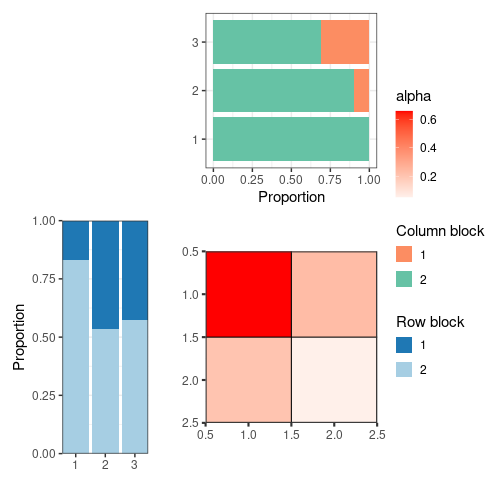
\includegraphics{figure/pirho_meso_plot-2.png}
\caption{Collection 2 - pirho}
\end{figure}

\begin{longtable}[]{@{}l@{}}
\toprule
Networks\tabularnewline
\midrule
\endhead
Benadi2013\_3(1340m)\tabularnewline
Trojelsgaard2015\_La Gomera\tabularnewline
CordenizPicanco2018\_SemiPast\tabularnewline
\bottomrule
\end{longtable}

Pour la collection 3

\begin{figure}
\centering
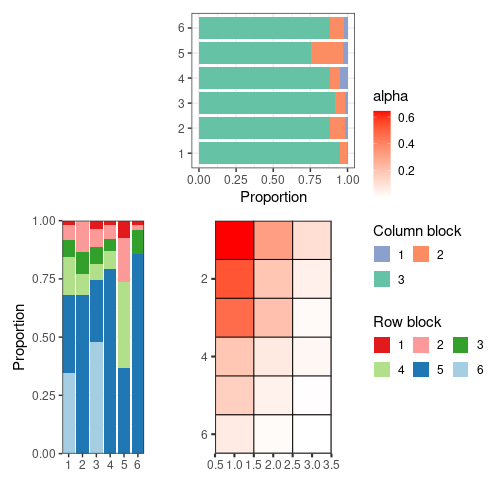
\includegraphics{figure/pirho_meso_plot-3.png}
\caption{Collection 3 - pirho}
\end{figure}

\begin{longtable}[]{@{}l@{}}
\toprule
Networks\tabularnewline
\midrule
\endhead
Kato2000\tabularnewline
Freitas2006\tabularnewline
Inoue1990\tabularnewline
Souza\_cerrado\tabularnewline
Adedoja2019\tabularnewline
Baldock2019\_Bristol\tabularnewline
\bottomrule
\end{longtable}

Pour la collection 4

\begin{figure}
\centering
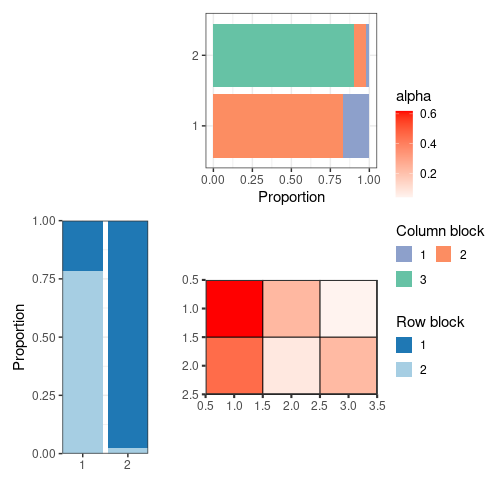
\includegraphics{figure/pirho_meso_plot-4.png}
\caption{Collection 4 - pirho}
\end{figure}

\begin{longtable}[]{@{}l@{}}
\toprule
Networks\tabularnewline
\midrule
\endhead
Aizen2008\_Puerto Blest\_U+Aizen2008\_Puerto Blest\_D\tabularnewline
LemusJimenez2003\tabularnewline
\bottomrule
\end{longtable}

Pour la collection 5

\begin{figure}
\centering
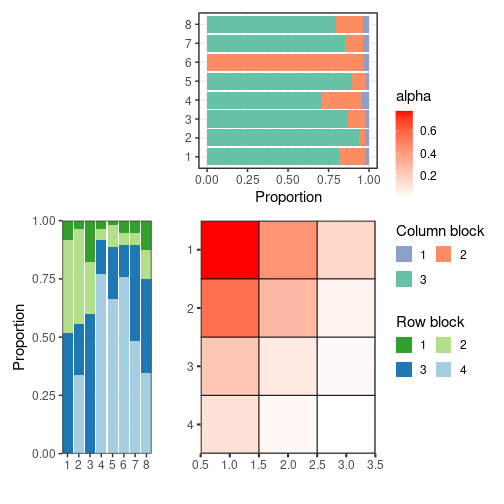
\includegraphics{figure/pirho_meso_plot-5.png}
\caption{Collection 5 - pirho}
\end{figure}

\begin{longtable}[]{@{}l@{}}
\toprule
Networks\tabularnewline
\midrule
\endhead
inouye1988\tabularnewline
Junker2013\tabularnewline
Kehinde2014\_Joostenberg\_Conv+Kehinde2014\_Joostenberg\_Org+Kehinde2014\_Joostenberg\_Nat+Kehinde2014\_Laibach\_Conv+Kehinde2014\_Laibach\_Org+Kehinde2014\_Laibach\_Nat+Kehinde2014\_Spier\_Conv+Kehinde2014\_Spier\_Nat\tabularnewline
Watts2016\_Chicon+Watts2016\_Mantanay+Watts2016\_Choquebamba+Watts2016\_Huaran+Watts2016\_Piscacucho+Watts2016\_Poques+Watts2016\_Pumamarca+Watts2016\_Tiaparo+Watts2016\_Yanacocha\tabularnewline
Kakutani1990\tabularnewline
Fragoso\_RA1+Fragoso\_RD2\tabularnewline
Souza\_chaco\tabularnewline
Oleques2019\tabularnewline
\bottomrule
\end{longtable}

Pour la collection 6

\begin{figure}
\centering
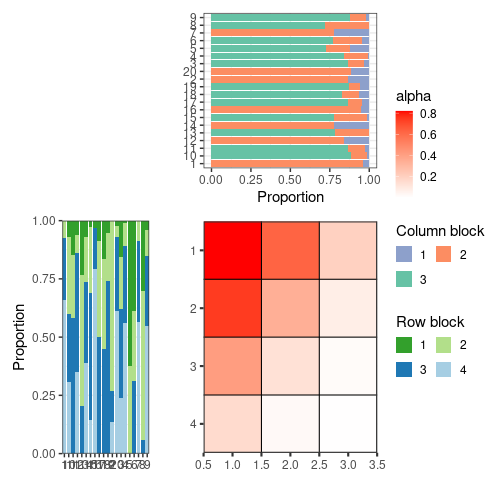
\includegraphics{figure/pirho_meso_plot-6.png}
\caption{Collection 6 - pirho}
\end{figure}

\begin{longtable}[]{@{}l@{}}
\toprule
Networks\tabularnewline
\midrule
\endhead
medan2002ld\tabularnewline
small1976\tabularnewline
smith-ramirez2005\tabularnewline
Benadi2013\_1(950m)+Benadi2013\_2(1170m)+Benadi2013\_6(2020m)\tabularnewline
Shay2016\tabularnewline
Aizen2008\_Cerro Otto\_U+Aizen2008\_Cerro Otto\_D\tabularnewline
Lundgren2005\tabularnewline
Zackenberg\tabularnewline
Carstensen\_Gigante+Carstensen\_Paulino+Carstensen\_Tinkerbell+Carstensen\_Midway+Carstensen\_Cedro+Carstensen\_Elefante+Carstensen\_Soizig\tabularnewline
Welti\_ID+Welti\_K1B+Welti\_K4A+Welti\_4B+Welti\_20B+Welti\_20C+Welti\_N1A+Welti\_N1B+Welti\_N4A+Welti\_N4B+Welti\_N20A+Welti\_N20B\tabularnewline
Bennett2018\tabularnewline
CordenizPicanco2018\_NatFor\tabularnewline
CordenizPicanco2018\_ExoFor\tabularnewline
CordenizPicanco2018\_IntPast\tabularnewline
Benadi2018\tabularnewline
Villalobos2019\tabularnewline
Traveset2013\_Santiago\tabularnewline
Traveset2013\_SantaCruz\tabularnewline
Son2019\_a1+Son2019\_a2+Son2019\_a3+Son2019\_a4+Son2019\_a5+Son2019\_a6+Son2019\_a7+Son2019\_a8+Son2019\_F1+Son2019\_F2+Son2019\_F3+Son2019\_F4+Son2019\_F5+Son2019\_F6+Son2019\_F7+Son2019\_F8\tabularnewline
Sritongchuay2019\_near+Sritongchuay2019\_far\tabularnewline
\bottomrule
\end{longtable}

Pour la collection 7

\begin{figure}
\centering
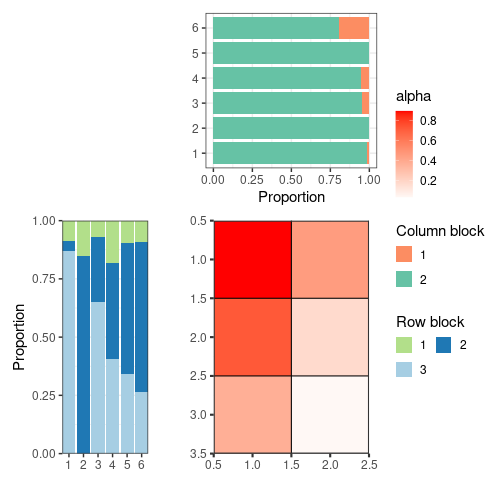
\includegraphics{figure/pirho_meso_plot-7.png}
\caption{Collection 7 - pirho}
\end{figure}

\begin{longtable}[]{@{}l@{}}
\toprule
Networks\tabularnewline
\midrule
\endhead
medan2002rb\tabularnewline
olensen2002flo\tabularnewline
vazquez2002\tabularnewline
Trojelsgaard2015\_Gran Canaria\tabularnewline
Trojelsgaard2015\_Western Sahara\tabularnewline
LaraRomero2019\_blanca+LaraRomero2019\_rajada+LaraRomero2019\_refugio+LaraRomero2019\_torre\tabularnewline
\bottomrule
\end{longtable}

Pour la collection 8

\begin{figure}
\centering
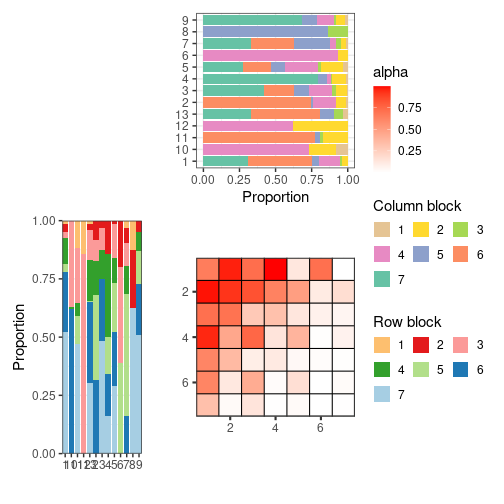
\includegraphics{figure/pirho_meso_plot-8.png}
\caption{Collection 8 - pirho}
\end{figure}

\begin{longtable}[]{@{}l@{}}
\toprule
Networks\tabularnewline
\midrule
\endhead
Weiner2011\tabularnewline
Kaiser\_control+Kaiser\_restored\tabularnewline
Gilarranz2014\_amarante+Gilarranz2014\_barrosa+Gilarranz2014\_cincocerros+Gilarranz2014\_difuntito+Gilarranz2014\_difuntos+Gilarranz2014\_elmorro+Gilarranz2014\_labrava+Gilarranz2014\_lachata+Gilarranz2014\_lapaja+Gilarranz2014\_piedraalta+Gilarranz2014\_vigilancia+Gilarranz2014\_volcan\tabularnewline
Kaiser-Bunbury2017\_Bernica+Kaiser-Bunbury2017\_Casse-dent+Kaiser-Bunbury2017\_Copolia+Kaiser-Bunbury2017\_La-Reserve+Kaiser-Bunbury2017\_Rosebelle+Kaiser-Bunbury2017\_Salazie+Kaiser-Bunbury2017\_Tea-Plantation+Kaiser-Bunbury2017\_Trois-Freres\tabularnewline
Fang2012\tabularnewline
Gibson2006\_SG\tabularnewline
Gibson2006\_TA1\tabularnewline
Trojelsgaard2015\_Fuerteventura\tabularnewline
Pfeiffer\_CNE+Pfeiffer\_CNM+Pfeiffer\_CNT+Pfeiffer\_CPB+Pfeiffer\_CPM+Pfeiffer\_CPR+Pfeiffer\_CPS+Pfeiffer\_M2+Pfeiffer\_RP1+Pfeiffer\_RP2+Pfeiffer\_LM+Pfeiffer\_LO+Pfeiffer\_BD+Pfeiffer\_BH+Pfeiffer\_BS\tabularnewline
Biella2019\tabularnewline
Nel2017\tabularnewline
Ferrero2013\tabularnewline
Neli2014\tabularnewline
\bottomrule
\end{longtable}

Pour la collection 9

\begin{figure}
\centering
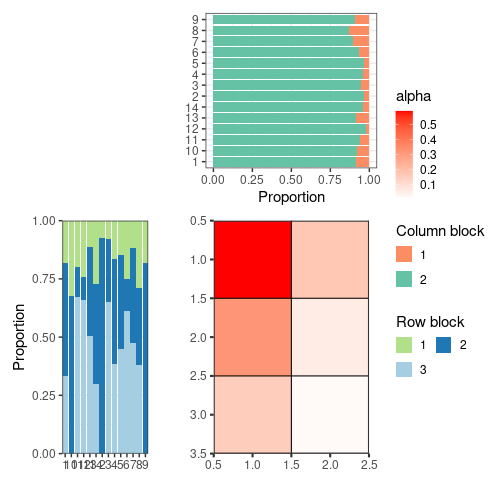
\includegraphics{figure/pirho_meso_plot-9.png}
\caption{Collection 9 - pirho}
\end{figure}

\begin{longtable}[]{@{}l@{}}
\toprule
Networks\tabularnewline
\midrule
\endhead
eberling1999\tabularnewline
ramirez1992\tabularnewline
Struck1994\tabularnewline
Albrecht2010\_49yr+Albrecht2010\_63yr+Albrecht2010\_84yr+Albrecht2010\_109yr+Albrecht2010\_130yr\tabularnewline
Devoto2005\_PP+Devoto2005\_AP\tabularnewline
Devoto2005\_VT\tabularnewline
Gibson2006\_TA2\tabularnewline
MonteroCastano2017\_Albufera+MonteroCastano2017\_Llimpa+MonteroCastano2017\_Tirant\tabularnewline
Yoshihara2008\tabularnewline
PopicThesis\tabularnewline
Orford\_B1+Orford\_B2+Orford\_B3+Orford\_B4+Orford\_B5+Orford\_B10\tabularnewline
Souza\_vereda\tabularnewline
Adedoja2018b\_baseZone+Adedoja2018b\_MidZone+Adedoja2018b\_HighZone+Adedoja2018b\_PeakZone\tabularnewline
Hackett2019\_NZ\_salt\_marsh+Hackett2019\_NZ\_sand\_dune+Hackett2019\_NZ\_scrub\_coprosma\tabularnewline
\bottomrule
\end{longtable}

Pour la collection 10

\begin{figure}
\centering
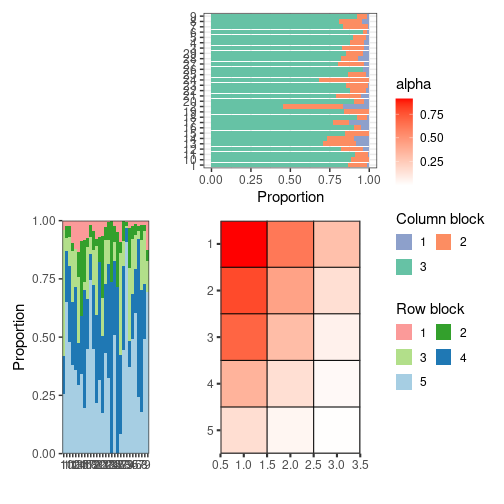
\includegraphics{figure/pirho_meso_plot-10.png}
\caption{Collection 10 - pirho}
\end{figure}

\begin{longtable}[]{@{}l@{}}
\toprule
Networks\tabularnewline
\midrule
\endhead
herrera1988\tabularnewline
Burkle2013\tabularnewline
bartomeus2008\tabularnewline
Olito-Fox2014\tabularnewline
Benadi2013\_4(1700m)+Benadi2013\_5(1800m)\tabularnewline
Baldock2011\_TB+Baldock2011\_JN\tabularnewline
Chamberlain\_HLU+Chamberlain\_HLG+Chamberlain\_OKU+Chamberlain\_OKG+Chamberlain\_WLU+Chamberlain\_WLG+Chamberlain\_SOU+Chamberlain\_SOG\tabularnewline
Chamberlain\_Site1+Chamberlain\_Site2+Chamberlain\_Site3+Chamberlain\_Site4+Chamberlain\_Site5+Chamberlain\_Site6\tabularnewline
Devoto2005\_LQ\tabularnewline
Devoto2005\_LT+Devoto2005\_LH\tabularnewline
Devoto2005\_LL+Devoto2005\_CT\tabularnewline
Dupont2009\_IsenBjerg+Dupont2009\_Other\tabularnewline
Gibson2006\_GA1\tabularnewline
LaraRomero2016\_pe?alara\_EP+LaraRomero2016\_pe?alara\_PA+LaraRomero2016\_nevero\_EP+LaraRomero2016\_nevero\_PA\tabularnewline
Marrero2013\tabularnewline
Trojelsgaard2015\_Tenerife Teno Bajo+Trojelsgaard2015\_Tenerife
Fasnia\tabularnewline
Vanbergen2013\_balfarm+Vanbergen2013\_bridgend+Vanbergen2013\_dalhaikie+Vanbergen2013\_netherton+Vanbergen2013\_backhill+Vanbergen2013\_corntulloch+Vanbergen2013\_allancreich\tabularnewline
Fragoso\_RA2+Fragoso\_RA3+Fragoso\_RD1+Fragoso\_RD3\tabularnewline
Pornon2017\tabularnewline
Orford\_B6+Orford\_B7+Orford\_B8+Orford\_B9\tabularnewline
Blumel2016\tabularnewline
Kantsa2018\tabularnewline
Grass2013\_1+Grass2013\_2+Grass2013\_3+Grass2013\_4+Grass2013\_5+Grass2013\_6+Grass2013\_7+Grass2013\_8+Grass2013\_9+Grass2013\_10+Grass2013\_11+Grass2013\_12+Grass2013\_13+Grass2013\_14+Grass2013\_15+Grass2013\_16+Grass2013\_17\tabularnewline
CordenizPicanco2018\_NatVeg\tabularnewline
Hackett2019\_UK\_sand\_dune+Hackett2019\_UK\_grassland+Hackett2019\_UK\_heathland+Hackett2019\_UK\_woodland+Hackett2019\_UK\_salt\_marsh+Hackett2019\_UK\_scrub\tabularnewline
Traveset2013\_Pinta\tabularnewline
Traveset2013\_SanCristobal\tabularnewline
Simanonok2014\tabularnewline
Baldock2019\_Edinburgh\tabularnewline
\bottomrule
\end{longtable}

Pour la collection 11

\begin{figure}
\centering
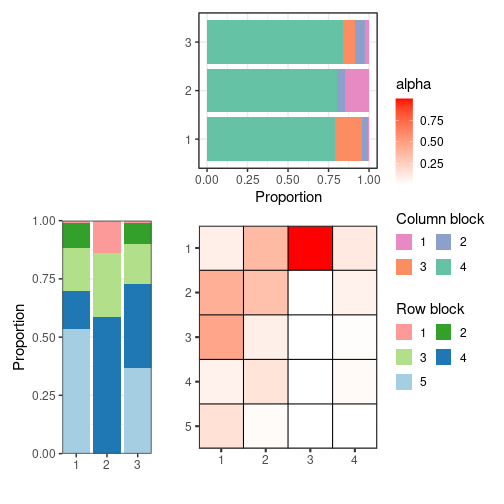
\includegraphics{figure/pirho_meso_plot-11.png}
\caption{Collection 11 - pirho}
\end{figure}

\begin{longtable}[]{@{}l@{}}
\toprule
Networks\tabularnewline
\midrule
\endhead
kato1990\tabularnewline
ramirez1989\tabularnewline
Kato1993\tabularnewline
\bottomrule
\end{longtable}

Pour la collection 12

\begin{figure}
\centering
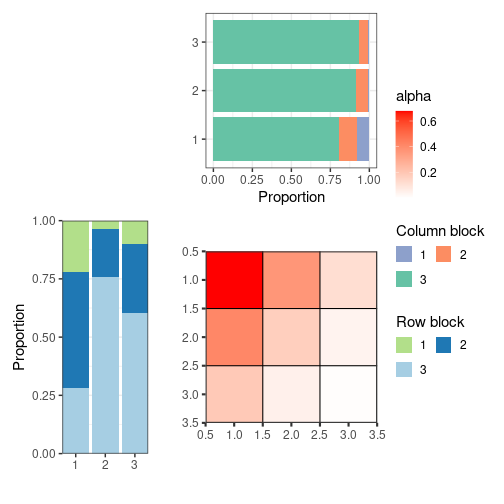
\includegraphics{figure/pirho_meso_plot-12.png}
\caption{Collection 12 - pirho}
\end{figure}

\begin{longtable}[]{@{}l@{}}
\toprule
Networks\tabularnewline
\midrule
\endhead
Chamberlain\_cr1+Chamberlain\_cr2+Chamberlain\_fs1+Chamberlain\_fs2+Chamberlain\_go1+Chamberlain\_go2+Chamberlain\_mm1+Chamberlain\_mm2+Chamberlain\_mz1+Chamberlain\_mz2+Chamberlain\_sm1+Chamberlain\_sm2\tabularnewline
Dattilo2016\tabularnewline
KatoMiura1996\tabularnewline
\bottomrule
\end{longtable}

Pour la collection 13

\begin{figure}
\centering
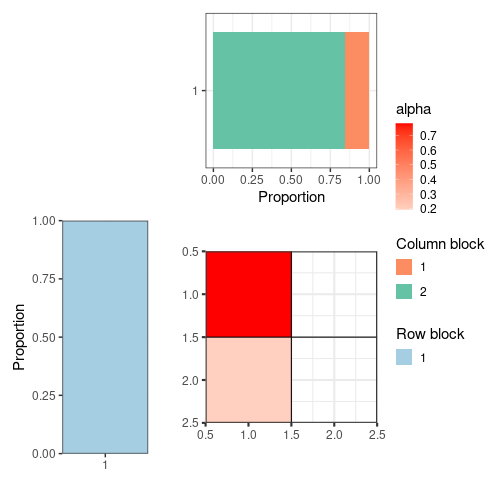
\includegraphics{figure/pirho_meso_plot-13.png}
\caption{Collection 13 - pirho}
\end{figure}

\begin{longtable}[]{@{}l@{}}
\toprule
Networks\tabularnewline
\midrule
\endhead
olensen2002aig\tabularnewline
\bottomrule
\end{longtable}

Pour la collection 14

\begin{figure}
\centering
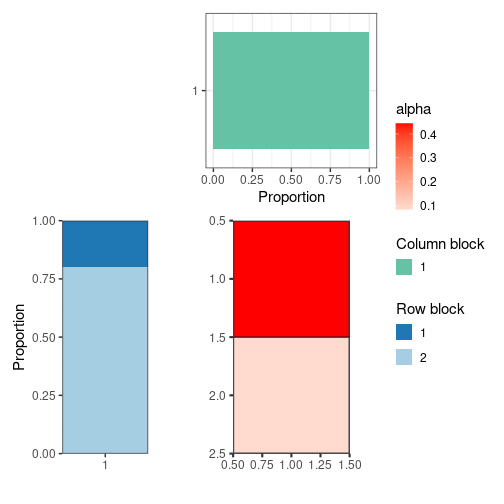
\includegraphics{figure/pirho_meso_plot-14.png}
\caption{Collection 14 - pirho}
\end{figure}

\begin{longtable}[]{@{}l@{}}
\toprule
Networks\tabularnewline
\midrule
\endhead
Trojelsgaard2015\_El Hierro\tabularnewline
\bottomrule
\end{longtable}

Pour la collection 15

\begin{figure}
\centering
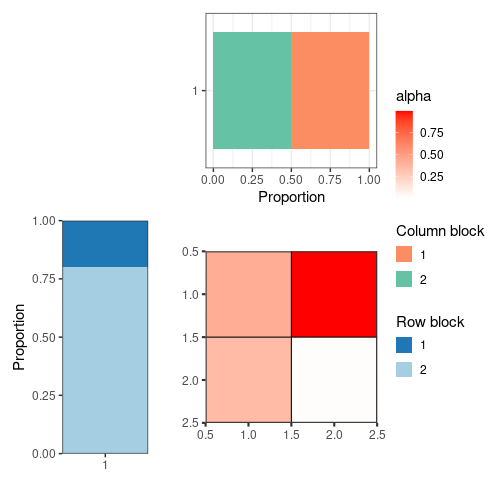
\includegraphics{figure/pirho_meso_plot-15.png}
\caption{Collection 15 - pirho}
\end{figure}

\begin{longtable}[]{@{}l@{}}
\toprule
Networks\tabularnewline
\midrule
\endhead
Gibson2006\_GA2\tabularnewline
\bottomrule
\end{longtable}

Et voici donc les valeurs numériques pour les \(\alpha\) (paramètres de
connectivité).

Pour la collection 1 :
\[\begin{bmatrix} 0.52 &0.6 &0.34 &0.1 &0.15 &0 &0.36 \\0.12 &0.93 &0.01 &0.01 &0 &0.61 &0.16 \\0.05 &0.31 &0.02 &0.08 &0.37 &0.27 &0.12 \\0.04 &0.05 &0.01 &0.38 &0.03 &0.01 &0.17 \\0 &0.03 &0.16 &0.11 &0.04 &0.01 &0.01 \\0.01 &0.22 &0.02 &0.01 &0.05 &0 &0.01 \\ \end{bmatrix}\]
Pour la collection 2 :
\[\begin{bmatrix} 0.66 &0.23 \\0.2 &0.05 \\ \end{bmatrix}\] Pour la
collection 3 :
\[\begin{bmatrix} 0.64 &0.32 &0.11 &0.53 &0.19 &0.05 \\0.47 &0.21 &0.02 &0.19 &0.07 &0.03 \\0.16 &0.05 &0.01 &0.07 &0.01 &0 \\ \end{bmatrix}\]
Pour la collection 4 :
\[\begin{bmatrix} 0.45 &0.07 \\0.22 &0.62 \\0.23 &0.04 \\ \end{bmatrix}\]
Pour la collection 5 :
\[\begin{bmatrix} 0.78 &0.43 &0.16 &0.56 \\0.29 &0.04 &0.22 &0.08 \\0.02 &0.12 &0.03 &0 \\ \end{bmatrix}\]
Pour la collection 6 :
\[\begin{bmatrix} 0.82 &0.63 &0.2 &0.74 \\0.34 &0.07 &0.41 &0.13 \\0.02 &0.16 &0.03 &0 \\ \end{bmatrix}\]
Pour la collection 7 :
\[\begin{bmatrix} 0.9 &0.46 &0.72 \\0.17 &0.37 &0.03 \\ \end{bmatrix}\]
Pour la collection 8 :
\[\begin{bmatrix} 0.66 &0.97 &0.72 &1 &0.13 &0.71 &0 \\0.99 &0.93 &0.84 &0.64 &0.5 &0.11 &0.17 \\0.71 &0.7 &0.28 &0.32 &0.13 &0.07 &0.05 \\0.96 &0.46 &0.75 &0.14 &0.39 &0.01 &0.07 \\0.62 &0.36 &0.09 &0.11 &0.04 &0.02 &0.01 \\0.62 &0.12 &0.43 &0.02 &0.17 &0 &0.02 \\0.33 &0.03 &0.14 &0 &0.03 &0 &0 \\ \end{bmatrix}\]
Pour la collection 9 :
\[\begin{bmatrix} 0.59 &0.17 &0.32 \\0.06 &0.15 &0.02 \\ \end{bmatrix}\]
Pour la collection 10 :
\[\begin{bmatrix} 0.91 &0.62 &0.3 &0.79 &0.44 \\0.15 &0.7 &0.32 &0.07 &0.36 \\0.15 &0.03 &0.16 &0.05 &0.01 \\ \end{bmatrix}\]
Pour la collection 11 :
\[\begin{bmatrix} 0.09 &0.36 &1 &0.12 &0.41 \\0.33 &0 &0.07 &0.46 &0.09 \\0 &0.01 &0.07 &0.14 &0 \\0.03 &0.16 &0.02 &0 &0 \\ \end{bmatrix}\]
Pour la collection 12 :
\[\begin{bmatrix} 0.68 &0.37 &0.12 \\0.41 &0.17 &0.04 \\0.19 &0.05 &0.01 \\ \end{bmatrix}\]
Pour la collection 13 : \[\begin{bmatrix} 0.78 \\0.19 \\ \end{bmatrix}\]
Pour la collection 14 : \[\begin{bmatrix} 0.44 &0.08 \\ \end{bmatrix}\]
Pour la collection 15 :
\[\begin{bmatrix} 0.42 &1 \\0.35 &0.01 \\ \end{bmatrix}\]

\hypertarget{ruxe9partition-dans-les-clusters-selon-la-taxonomie-3}{%
\subsubsection{Répartition dans les clusters selon la
taxonomie}\label{ruxe9partition-dans-les-clusters-selon-la-taxonomie-3}}

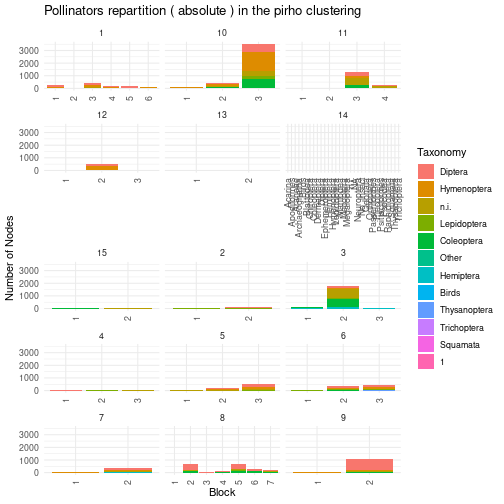
\includegraphics{figure/pirho_plot_taxonomy_pollinators-1.png}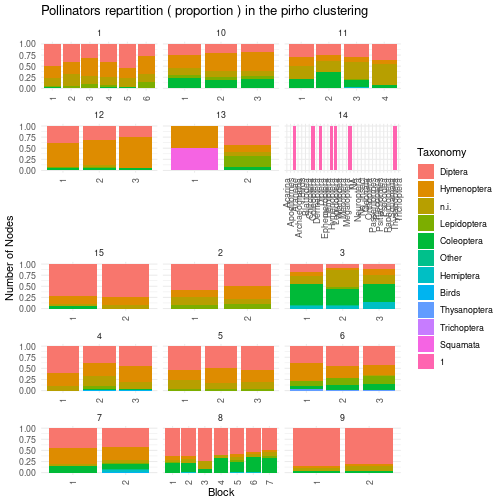
\includegraphics{figure/pirho_plot_taxonomy_pollinators-2.png}

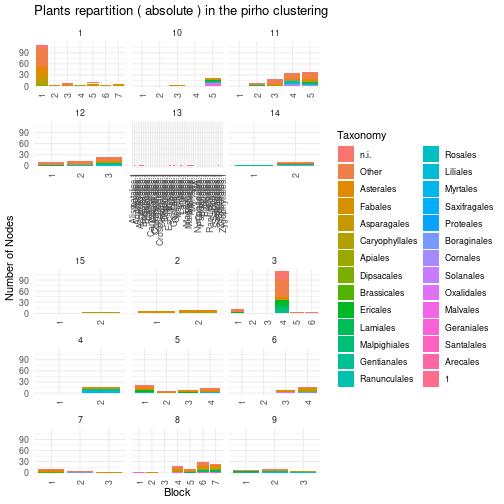
\includegraphics{figure/pirho_plot_taxonomy_plants-1.png}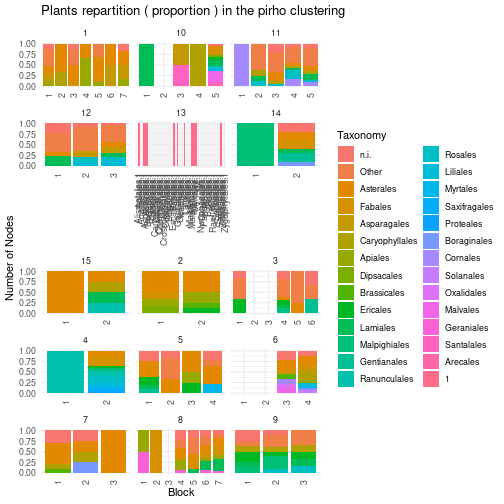
\includegraphics{figure/pirho_plot_taxonomy_plants-2.png}
